\section{DC Servomotor}\label{sec:servo_motor}

The control of both antennas requires the use of four motors which will be able to change its orientation (two motors per antenna in order to control two different angles). The DC servomotor can be either a rotary or a linear actuator. In this project, a rotary servomotor was chosen because it allows a precise control of angular position, velocity and acceleration.

The servomotor can be described in two different parts: an electrical motor and a servomechanism. The electrical motor is a DC motor which is able to convert electrical power into rotational mechanical power and the servomechanism is the group of elements connected with the DC motor. The shaft of the DC motor is coupled with another shaft denominated output shaft. The connection is made through a gear assembly which is not only responsible for the connection between both shafts, but also for the reduction of the RPM of the motor’s shaft (figure \ref{servomotor_expl1}).

\begin{figure}[H]
\centering
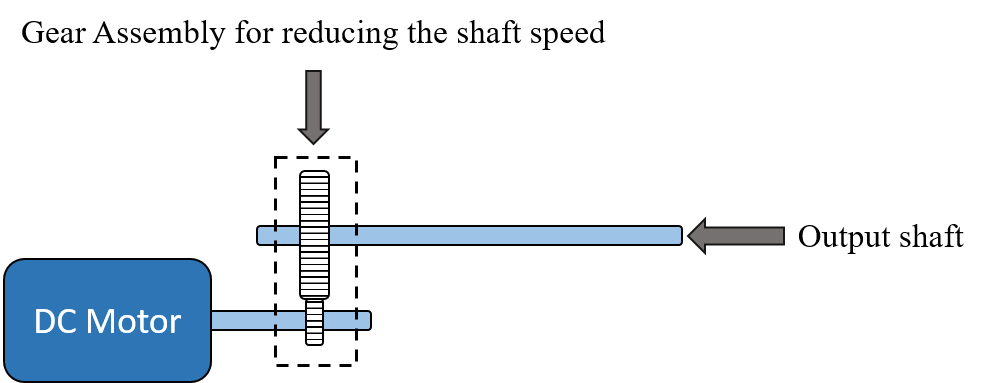
\includegraphics[scale=0.7]{figures/servomotor_expl1.png}
\caption{Connection between the output shaft and the DC motor}
\label{servomotor_expl1}
\end{figure}

The output shaft is also connected with a potentiometer by another gear assembly and, during its rotation, the knob rotates and creates an electrical signal. This signal increases proportionally with the angular movement of the potentiometer knob. The connection between the output shaft and the potentiometer can be
observed in the figure \ref{servomotor_expl2}.

\begin{figure}[H]
\centering
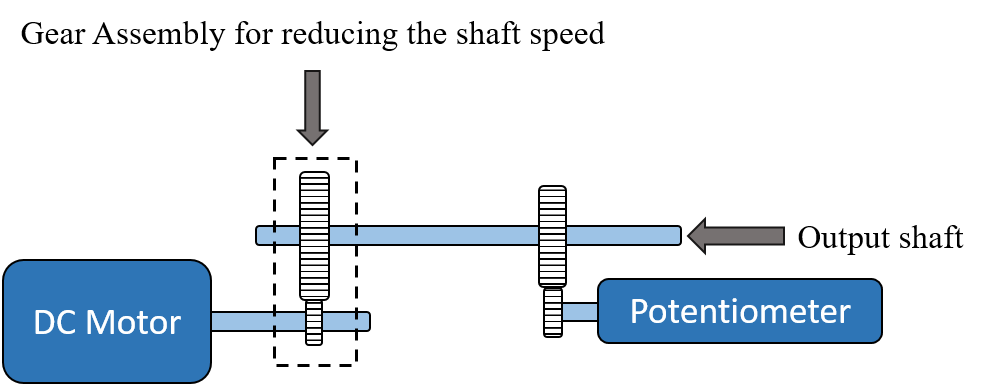
\includegraphics[scale=0.61]{figures/servomotor_expl2.png}
\caption{Connection between the output shaft and the potentiometer}
\label{servomotor_expl2}
\end{figure}

The previous described gears are involved in the gear mechanism which is responsible for the transformation of the original input speed provided by the DC motor into a slower output speed which is practical and widely applicable. 

The potentiometer is also connected with an error detector feedback amplifier where the electrical potential (from the potentiometer) and the input command voltage (the signal that represents the desired angle) are compared. The output of the error detector amplifier is called electrical input of the DC motor and is represented in the figure \ref{servomotor_expl3}. When the electrical potential equals the input voltage, which means that the shaft is in the desired position, the input of the DC motor becomes zero and the motor stops rotating until the next command.

\begin{figure}[H]
\centerline{
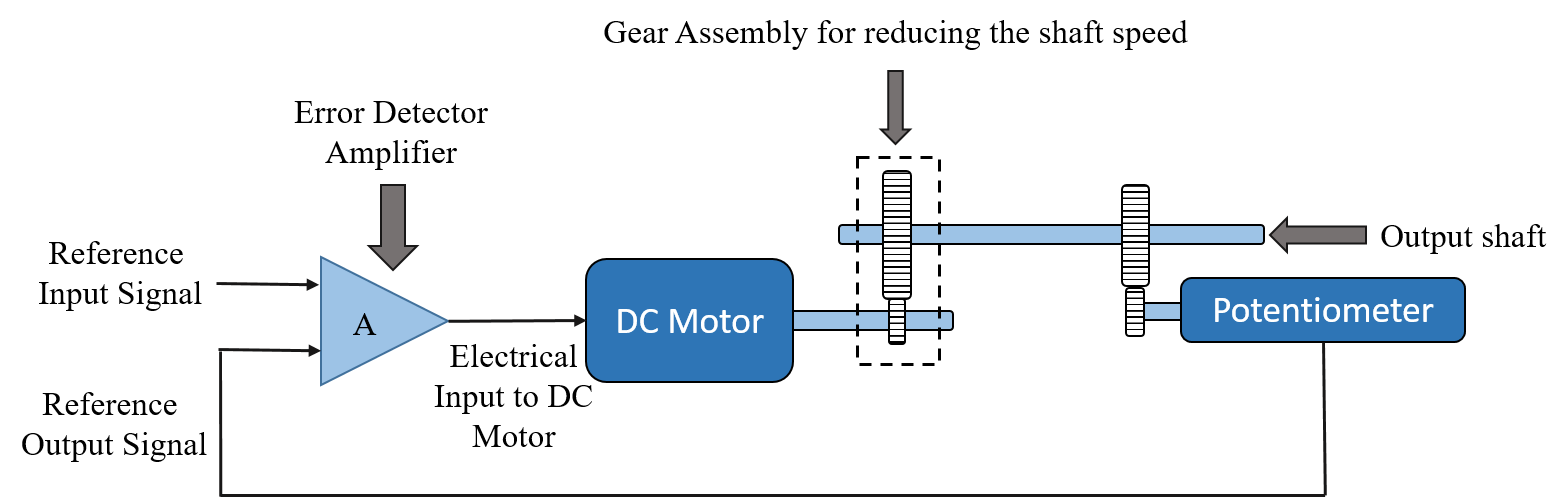
\includegraphics[scale=0.6]{figures/servomotor_expl3new.png}}
\caption{Servomotor’s feedback}
\label{servomotor_expl3}
\end{figure}

In order to be able to do the procedure described in the figure \ref{servomotor_expl3} it is necessary to apply a restricted input voltage signal in regular intervals. Servomotors operate from 4.8V to a 6V supply voltage, but 5V is the typical value. Furthermore, the pulse should have a specific width (PWM – Pulse Width Modulation) because it will be responsible for the amount of rotation. Typically, the duration of the pulse varies from 1ms to 2.2ms and the frequency from 50Hz to 60Hz. The size of the pulse will result in a lesser or greater rotation. The figure \ref{signal_servo} is an example of the relation pulse-rotation and describes three different cases. For instance, if the duration of the pulse is 1.25ms, the servomotor will rotate 90 degrees.

\begin{figure}[H]
\centering
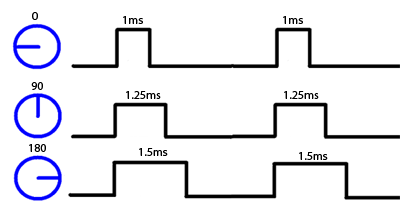
\includegraphics[scale=0.5]{figures/signal_servo.jpg}
\caption{Examples of the relation between the PWM and the rotation}
\label{signal_servo}
\end{figure}

Based on the previous explanation, the servomotor requires a power supply unit and the information about the rotation that should be done through an electrical signal. Hence, this motor needs three different terminals (the figure \ref{cable_servo} is one example of the terminals of a servo motor):
\begin{itemize}  
        \item Yellow - Position signal (PWM pulses).
        \item Red - $V_{cc}$ (from the power supply unit). 
        \item Black - Ground.
\end{itemize}

\begin{figure}[H]
\centering
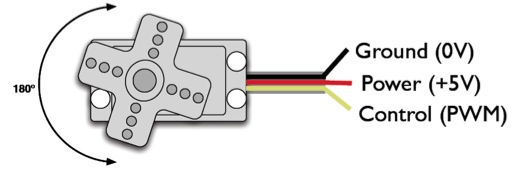
\includegraphics[scale=0.7]{figures/cable_servo.jpg}
\caption{Servo motor with its three different terminals}
\label{cable_servo}
\end{figure}

